\subsection{Light Collection for the Prompt Scintillation Signal (S1)}
\label{secLCEs1}

In order to calculate the position dependent light collection efficiency (LCE) for the prompt scintillation signal (S1), a Monte Carlo simulation has been performed with GEANT4. 
The S1 signal has been modeled with a point source of UV-photons with an energy of 7~eV, corresponding to the wavelength of 175~nm, placed uniformly at random positions within the liquid xenon volume. In total, 100'000 events have been simulated, with 10'000 photons generated each event.

Photon transportation in GEANT4 takes into account the light absorption and Rayleigh scattering in the liquid and gaseous xenon, and reflection and refraction at the optical surfaces. The results of the simulation significantly depend on the optical parameters of different materials used for the light propagation. The assumed parameters are listed in Table~\ref{tabOpticalParameters}. The reflection distribution of PTFE 
 has been modeled by including both diffuse and specular lobes, based on available measurements~\cite{TeflonReflection}. However, it is subject to large uncertainties, as it depends on how the surfaces are machined.
 % The refractive index for electrode meshes is set equal to that of LXe.

\begin{table}[!h]
\centering
\caption{Optical parameters for the different materials, used in the Monte Carlo simulations of the light collection with GEANT4.}
\label{tabOpticalParameters}
%\vspace{0.2cm}
\begin{tabular}{>{\footnotesize}l |>{\footnotesize} l}
%\begin{tabular}{l|l}
\hline
Parameter						& Value \\
\hline
Liquid xenon absorption length 			& 1~m \\
Liquid xenon Rayleigh scattering length		& 30~cm \\
Liquid xenon refractive index				& 1.63 \\
Gaseous xenon absorption length 			& 100~m \\
Gaseous xenon Rayleigh scattering length 	& 100~m \\
Photocathode refractive index 				& 1.50 \\
Photocathode absorption length 			& 1~nm \\
Quartz (synthetic silica) refractive index 		& 1.50 \\
Quartz (synthetic silica) absorption length 	& 30~m \\
Teflon refractive index 					& 1.63 \\
Teflon reflectivity 						& 95\% \\
Steel reflectivity 						& 20\% \\
Copper reflectivity						& 20\% \\
Electrode mesh absorption length			& 2.10~mm \\
\hline
\end{tabular}
\end{table}


The LCE is defined as the ratio of the total number of photons hitting the PMTs and the total number of the photons emitted at each point. The LCE for S1 in the target and veto liquid xenon volumes is presented as a function of the event location in Fig.~\ref{figLCEmapsS1}. The average LCE in the target volume is 24\%, and 4.7\% in the veto. Due to total reflection of the light at the liquid-gas interface, most of S1 light is detected by the bottom array. The S1 signal detection by the top PMT array is very low, and does not exceed $\sim$10\% even for events close to the liquid surface~(Fig.~\ref{figLCEmapsS1_3}). 
%The dashed lines in Fig.~\ref{figLCEmapsS1_2} show the location of the top meshes (three lines at the top of the target volume) and positions of the cathode and the synthetic silica window of the bottom PMTs (two lines at the bottom of the target volume).

%In the region between the cathode and a PMT window, which is 18~mm thick ($\sim$4~kg of liquid xenon), the electric field is reversed, and the ionization electrons are drifted in the opposite direction and do not produce proportional scintillation signal which can be detected. Thus, this region is charge insensitive, and can be a source of so-called 'gamma-X' events. Such events happen when a gamma has two or more interactions in the LXe, one of which is in the region below the cathode. This results in a loss of some portion of the ionization signal, whereas scintillation produced in all interactions is detected. This leads to an abnormally low (non-Gaussian) value of the discrimination parameter log$_{10}$(S2/S1), which can mimic the nuclear recoil signal expected from a WIMP.

The results of the Monte Carlo simulation have been compared to the detector performance measured with a $^{137}$Cs source by means of the relative S1 collection efficiency. The target volume has been divided into different regions according to {\it Z} coordinate (or drift time), and the LCE distribution in each slice has been fitted with a Gaussian function. The resulting  distribution has been fitted with a polynomial function of the 5th degree and normalized to the maximum LCE value, which is calculated for the region at the very bottom of the target volume. As shown in Fig.~\ref{figLCEdataMC_1}, the relative LCE for S1 signal calculated for Monte Carlo and measured data are in a good agreement, and deviation of $\sim$20\% can be seen only at the very small drift times, close to the liquid surface.

\begin{figure}[!h]
\centering
\subfigure[]{
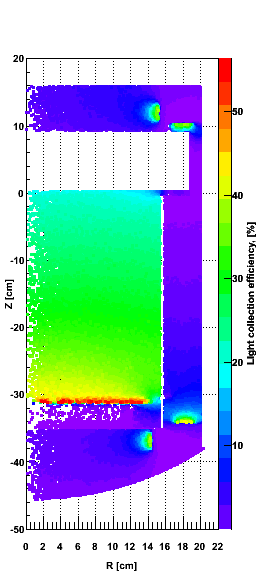
\includegraphics[height=0.6\linewidth]{plots/LCEs1/RZhits.png}
\label{figLCEmapsS1_1}}
\subfigure[]{
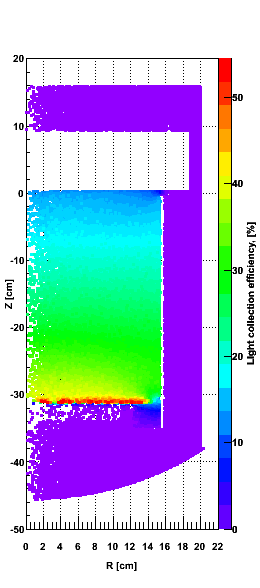
\includegraphics[height=0.6\linewidth]{plots/LCEs1/RZhitsBot_target.png}
\label{figLCEmapsS1_2}}
\subfigure[]{
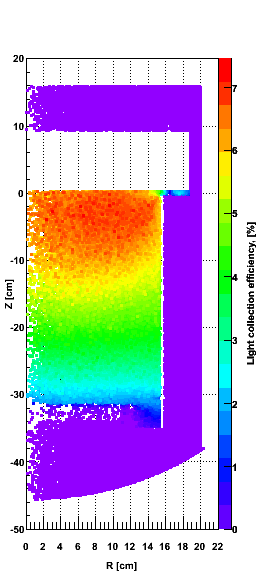
\includegraphics[height=0.6\linewidth]{plots/LCEs1/RZhitsTop_target.png}
\label{figLCEmapsS1_3}}
\caption[Detection efficiency for prompt scintillation signal (S1) simulated with GEANT4]{Detection efficiency for prompt scintillation signal (S1) simulated with GEANT4: (a) - combined LCE in the target and veto volumes; (b) - LCE by the bottom PMT array in the target volume; (c) - LCE by the top PMT array in the target volume. The quantum and collection efficiency of the PMTs are not included.}
\label{figLCEmapsS1}
\end{figure}

\begin{figure}[!h]
\centering
\subfigure[]{
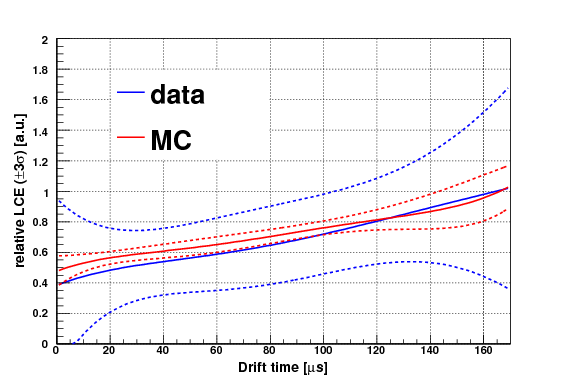
\includegraphics[width=0.475\linewidth]{plots/LCEs1/LCE_MCandData.png}
\label{figLCEdataMC_1}}
\subfigure[]{
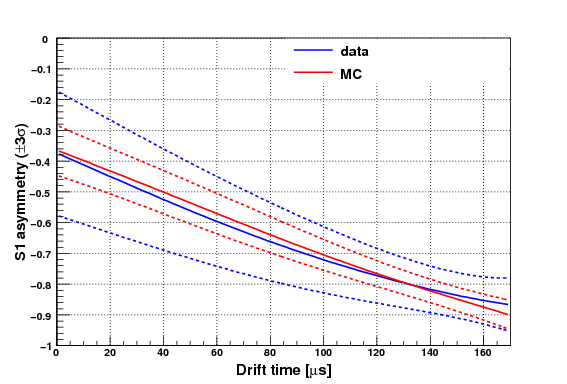
\includegraphics[width=0.475\linewidth]{plots/LCEs1/S1asym_MCandData.png}
\label{figLCEdataMC_2}}
\caption[Relative collection efficiency and asymmetry for S1 signal in Monte Carlo simulation and $^{137}$Cs data]{Relative collection efficiency (a) and asymmetry (b) for S1 signal in Monte Carlo simulation and $^{137}$Cs calibration data. The mean value and 3$\sigma$ contours are shown with solid and dashed lines, respectively. For large drift times, measurement and simulation are in a very good agreement  .}
\label{figLCEdataMC}
\end{figure}

An important parameter that can be calculated for the S1 signal is its top-bottom asymmetry, defined as:
\begin{equation}
\mathrm{S}1_{\mathrm{asymmetry}} = \frac{\mathrm{S}1_{\mathrm{top}} \-- \mathrm{S}1_{\mathrm{bottom}}}{\mathrm{S}1_{\mathrm{top}} + \mathrm{S}1_{\mathrm{bottom}}}.
\end{equation}
 
It can be used cross-check the depth of the interaction inferred from delay time between S2 and S1 signals, and to approximately determine the {\it Z} coordinate of an event, when drift time information between an S1 and a corresponding S2 is not available, for example, in single phase operation mode.

The S1 asymmetry parameter in the target volume has been calculated for Monte Carlo and $^{137}$Cs calibration data, for different {\it Z}-slices of 10~$\mu$s each. The distribution in each slice has been fitted with a Gaussian function. The mean of the Gaussian distribution and $\pm$3$\sigma$ contours are shown as a function of the drift time in Fig.~\ref{figLCEdataMC_2}. The fit has been performed with polynomial function of the 5th degree. The S1 asymmetry in the simulation agrees very well with the measurement.

A 3D map of the S1 LCE, which is mandatory to correct the data, has been obtained with three different radioactive sources: an external $^{137}$Cs $\gamma$-source (662~keV) taken with the lower field in the proportional scintillation region (0.25-0.30~kV/cm$^{2}$) in order to avoid non-linearity effects in the PMT (see Section~\ref{secPosRecSaturation}) at different positions around the detector, the 40~keV from inelastic scattering of neutrons on $^{129}$Xe, and the 164~keV line from neutron-activated $^{131\mathrm{m}}$Xe with a uniform distribution inside the TPC.

%\begin{floatingfigure}[l]{0.6\textwidth}
\begin{figure}[!h]
\centering
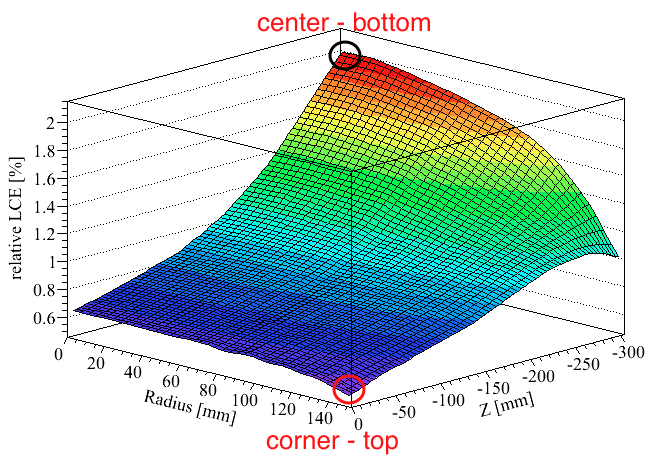
\includegraphics[width=0.6\linewidth]{plots/LCEs1/S1correctionMap_withLabels.png}
\caption[3D spatial correction map for S1, obtained for 40~keV $\gamma$-line]{3D spatial correction map for S1, obtained for 40~keV $\gamma$-line. Figure from Ref.~\cite{xe100-instrument}.}
\label{figCorrectionMapS1}
\end{figure}
%\end{floatingfigure}

For each of the sources, the peak position has been determined in $RZ$ bins with the smaller bin size at larger $R$, where the LCE falls off stronger. The LCE map obtained for the 40~keV de-excitation line from inelastic neutron scatters on xenon nuclei is shown in Fig.~\ref{figCorrectionMapS1}. The results of the three measurements agree within 3\%. As expected from Monte Carlo simulations, the LCE varies by almost a factor 3 across the TPC, with the largest value in the center, right above the bottom PMT array, and the minimum at large $R$, just below the gate grid.




